\chapter[Publication I]{Seasonal gene expression profiling of Antarctic krill
in three different latitudinal regions}

Flavia Höring, Lars Harms, Cristiano De Pittà, Gabriele Sales, Christian Reiss,
Bettina Meyer

Ready to be submitted to the journal Marine Genomics

\section*{Abstract}
The key organism Antarctic krill, \textit{Euphausia superba}, has evolved
seasonal rhythms of physiology and behaviour to survive under the extreme
photoperiodic conditions in the Southern Ocean. However, the molecular
mechanisms generating these rhythms remain far from understood. The aim of this
study was to investigate seasonal and regional differences in gene expression
in three different latitudinal regions with variable photoperiodic conditions
(South Georgia, South Orkneys/Bransfield Strait, Lazarev Sea) and to identify
genes with potential regulatory roles in the seasonal life cycle of Antarctic
krill. The RNAseq data were analysed (a) for seasonal differences
between summer and winter field samples from each region, and (b) for
regional differences within each season. In general, we found an upregulation
of gene expression in summer krill in all regions with respect to winter.
However, seasonal differences in gene expression were less pronounced in
Antarctic krill from South Georgia where most genes related to metabolic,
biological and regulatory processes were not found to be differentially
expressed between summer and winter krill. We also identified genes with
putative regulatory roles, for instance genes related to hormone metabolism and
signalling, reproductive and developmental processes. Our results suggest that
Antarctic krill entered a state of metabolic depression and regressed
development (so called winter quiescence) in South Orkneys/Bransfield Strait
and Lazarev Sea region in winter. The winter quiescence seems to be less
pronounced in the South Georgia region, most likely due to the milder seasonal
conditions, the less extreme light regime in this low-latitude region, and
hence food availability. These findings including the proposed target genes
provide a basis for future laboratory studies of the molecular mechanisms of
seasonal rhythms in Antarctic krill.

\section{Introduction}

Seasonal rhythms of physiology and behaviour are essential for the survival of
marine organisms inhabiting regions with extreme seasonal changes of
photoperiod (day length) like the Southern Ocean. Antarctic krill,
\textit{Euphausia superba}, holds a pivotal position in the Southern Ocean food
web where it is a major link between primary production and higher trophic
levels. It has been proposed that Antarctic krill may serve as a polar model
organism to study the effects of climate change in the polar ecosystem of the
Southern Ocean (Meyer, 2010). For that purpose, we want to understand the
mechanisms of its seasonal life cycle including its flexibility under changing
environmental conditions.

In the field, pronounced seasonal differences have been found in the Antarctic
krill's body composition, metabolic activity, feeding, growth (Meyer et al.,
2010) and maturity (Siegel, 2012). Survival in periods of near-constant
darkness and low food availability is accomplished by different overwintering
strategies. These include the accumulation of lipid reserves during summer and
the reduction of metabolic activity, feeding activity and growth (Meyer, 2012)
and sexual regression during winter.

Only few studies have investigated regional differences in the life cycle of
krill such as the timing of reproduction (Spiridonov, 1995) and growth
(Kawaguchi et al., 2006). Overwintering strategies seem to vary according to
latitudinal habitat as krill near South Georgia was observed to have lower
lipid stores and higher feeding activity in winter compared to higher
latitudinal regions (Schmidt et al., 2014). Seasonal and regional differences
in gene expression were found, for the first time, by Seear et al. (2012) who
investigated seasonal effects near the Antarctic Peninsula (\SI{60}{\degree}S) and
spatial differences in winter comparing the Antarctic Peninsula and South
Georgia (\SI{54}{\degree}S) region. This study concluded that genes involved in
feeding and digestion, respiration, motor activity, immunity and vitellogenesis
were upregulated in krill sampled in the Peninsula region during summer with
respect to winter. The regional comparison of winter krill revealed an
upregulation of genes related to feeding and digestion and immunity at South
Georgia compared to the Peninsula region.

The seasonal cycle of Antarctic krill is influenced by different environmental
factors such as light regime, food availability and/or temperature that may
contribute to krill's flexible behaviour in different latitudinal regions.
Controlled lab experiments have demonstrated the effect of temperature and food
supply on krill growth (Buchholz 1991) and maturity (Kawaguchi et al. 2007).
Photoperiod has been shown to affect feeding and metabolic activity (Teschke et
al., 2007), growth (Brown et al., 2010), maturity (Brown et al., 2011) and gene
expression (Seear et al., 2009) in Antarctic krill under laboratory conditions.
Based on the photoperiodic studies, it has been suggested that seasonal rhythms
in Antarctic krill are governed by an endogenous timing system with photoperiod
as Zeitgeber. Recently, it has been confirmed in a two-year lab experiment that
krill's seasonal rhythms seem to be affected by different latitudinal light
regimes (Höring et al., 2018).

Studies on the molecular mechanisms of the endogenous timing system in
Antarctic krill have mostly focused on daily rhythms, the circadian clock and
the photoperception system in \textit{E. superba}  (Biscontin et al., 2016,
2017; De Pittà et al., 2013; Piccolin et al., 2018a). Biscontin et al. (2016)
identified the opsin repertoire of Antarctic krill which may contribute to the
perception of daily and seasonal changes in irradiance and spectral composition
in the Southern Ocean. Antarctic krill possesses an ancestral circadian clock
machinery with both insect- and vertebrate like features and a light mediated
entraining mechanism (Biscontin et al., 2017). It has been suggested that
krill's circadian clock does not only control daily rhythms in \textit{E.
superba}, but may also be involved in the timing of seasonal life cycle events
(Piccolin et al., 2018b).

The flexibility of krill's seasonal cycle in different latitudinal regions and
the underlying molecular mechanisms are still poorly understood. Current
knowledge on the seasonal behaviour of Antarctic krill in the field is based on
single observations and the analysis of few regions, whereas data from the
winter season is generally less frequent. Even though extensive transcriptome
studies have been conducted in \textit{E. superba} (Meyer et al., 2015; Sales et
al., 2017), we still lack a comprehensive understanding of the molecular
pathways that contribute to the regulation of seasonal rhythms in Antarctic
krill in different latitudinal regions of the Southern Ocean. 

This paper aims to investigate seasonal and regional differences in gene
expression in Antarctic krill in three different latitudinal regions of the
Southern Ocean: South Georgia (\SI{54}{\degree}S), South Orkneys/Bransfield
Strait (\SI{60}{\degree}S-\SI{63}{\degree}S) and Lazarev Sea
(\SI{62}{\degree}S-\SI{66}{\degree}S). An RNA-seq approach is used to test for
(1) seasonal differences in gene expression between summer and winter krill
from each region, and (2) regional differences in gene expression between the
three different regional krill samples from each season. The RNA-seq data is
analysed with the goal to identify seasonal target genes with putative
regulatory functions in the seasonal life cycle of Antarctic krill.

\section{Methods}

\subsection*{Sample collection and experimental design}

Antarctic krill samples (\textit{Euphausia superba}) were obtained from five
different expeditions and from a Norwegian fishing vessel (Table I, Fig. \ref{Pub1_1}.
Sampling was carried out with a Rectangular Midwater Trawl (RMT8+1 for
expeditions ANT23-2, ANT23-6 and JR15004, RMT8 for expedition JR260B), an
Isaacs-Kidd Midwater Trawl (IKMT, expedition AMLR14) and a continuous pumping
system (Norwegian fishing vessel). Snap-frozen Antarctic krill samples stored
at \SI{-80}{\celsius} were transferred to the Alfred-Wegener-Institute, Bremerhaven,
for molecular analysis.

% Figure 1
\begin{figure}
        \caption{Station map indicating station numbers (NFV - Norwegian
        fishing vessel) and the three studied regions}
        \centering
        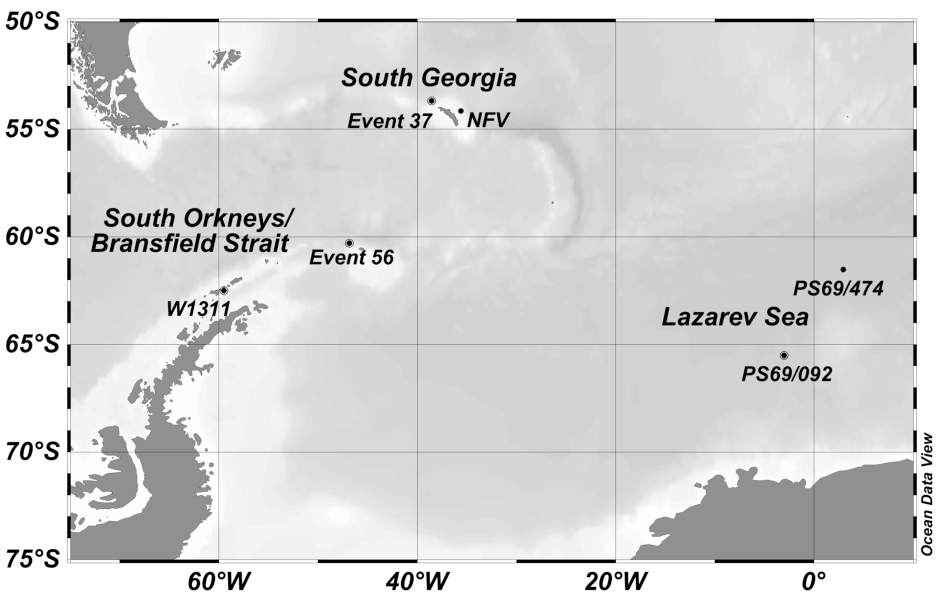
\includegraphics[width=0.85\textwidth]{../Figures/Pub1_1.pdf}
        \label{Pub1_1}
\end{figure}

The Antarctic krill originated from three different latitudinal regions:
a) Lazarev Sea (\SI{62}{\degree}S-\SI{66}{\degree}S), b) South
Orkneys/Bransfield Strait (\SI{60}{\degree}S-\SI{63}{\degree}S), and c) South
Georgia (\SI{54}{\degree}S), including summer and winter samples for each region.
By visual inspection of the outer sexual organs, male petasma and female
thelycum, adult males and females were identified. In total, 36 individuals
were chosen for further analysis, with 6-7 individuals for each regional and
seasonal sample including 3-4 females and 3 males (except the South Georgia
winter sample, where solely males were available, and 5 males were analysed;
see Table I for full sampling scheme).

\subsection*{RNA extraction, library preparation and Illumina sequencing}

RNA extraction was performed from frozen krill heads with the RNeasy Midi Kit
(QIAGEN, Hilden, Germany). Frozen krill heads were cut on dry ice and
transferred to \SI{1.5}{\milli\litre} RLT lysis buffer in tissue homogenizing
Precellys\textsuperscript{\textregistered} tubes (CKMix Tissue Homogenizing
Kit, Bertin corp., Rockville, MD, USA).  Homogenization was carried out at
\SI{4}{\celsius} in a Precellys\textsuperscript{\textregistered} homogenizer
with the Cryolys\textsuperscript{\textregistered} cooling system (Bertin corp.)
with two runs for \SI{15}{\second} at 5000 rpm and \SI{10}{\second} break.
Further steps of RNA extraction were carried out according to the
manufacturer's protocol of the RNeasy Midi Kit. The quality and quantity of the
RNA was inspected using the NanoDrop\texttrademark 2000 UV-Vis Spectrophotometer
(Thermo Fisher Scientific, Waltham, MA, USA) and the Agilent 2100 Bioanalyzer
system (Agilent technologies, Santa Clara, CA, USA).

RNA samples were sent for sequencing to IGA Technology Services (Udine, Italy).
cDNA libraries were performed with \SIrange{1}{2}{\micro\gram} RNA by using the
TruSeq Stranded mRNA Sample Prep kit (Illumina, San Diego, CA, USA) following
the manufacturer's instructions. The poly-A mRNA was fragmented 3 minutes at
\SI{94}{\celsius}. 1X Agencourt AMPure XP beads (Agencourt Bioscience Cooperation,
Beckman Coulter, Beverly, MA, USA) were used for every purification step. The
RNA samples and final cDNA libraries were quantified with the Qubit 2.0
Fluorometer (Invitrogen, Carlsbad, CA, USA) and quality tested by Agilent 2100
Bioanalyzer Nano assay.  For cluster generation on the flow cell, libraries
were processed with cBot (Illumina, San Diego, CA, USA) following
manufacturer's instructions.  Sequencing was carried out on paired-end mode
(2 $\times$ 100 bp) on HiSeq2500 (Illumina) with a targeted sequencing depth of about 80
million reads per sample. Raw data were processed with the software \code{CASAVA
v1.8.2} (Illumina) for both format conversion and de-multiplexing.

\subsection*{Quality control and analysis of RNA-seq data}

The programme \code{BBDuk} from \code{BBMap package v36.38} (Bushnell, 2016)
was used for the removal of adapter sequences and quality trimming of reads
(set parameters: ktrim=r, k=23, mink=11, hdist=1, tpe tbo, qtrim=r, trimq=10,
minlen=36). The quality of the trimmed reads was checked with the programme
\code{FastQC v0.11.5} (Andrews, 2017). Since the \code{FastQC} reports
indicated the presence of reads encoding ribosomal RNA, these reads were
removed using the software \code{SortMeRNA v2.1} (Kopylova et al., 2012). Transcript
abundance in each sample was estimated by aligning the processed paired-end
reads to the \textit{E. superba} reference transcriptome (Meyer et al., 2015)
using the software \code{Trinity v2.4.0} (Grabherr et al., 2011) with the
abundance estimation method \code{RSEM v1.2.26} (Li and Dewey, 2011) and the
alignment tool \code{Bowtie2 v2.2.5} (Langmead and Salzberg, 2012). As
reference, we chose the transcriptome by Meyer et al. (2015) instead of the
recently developed KrillDB transcriptome (Sales et al., 2017), because
preliminary alignment tests yielded approximately 10\% higher alignment rates
to the transcriptome by Meyer et al. (2015). Both transcript expression matrix
of non-normalized counts and matrix of TMM-normalized expression values were
calculated. Mapping rates to the reference transcriptome had a mean $\pm$ SD of
$69.22 \pm 3.37$\%. Differential gene expression was analysed with \code{edgeR}
(Robinson et al., 2010). Significant differentially expressed genes (DEGs) were
identified using a false discovery rate (FDR) cutoff value of $0.001$ and a
minimum absolute Log2 fold change (log2FC) of 2. Pairwise comparisons included
seasonal comparisons within each region and regional comparisons in both summer
and winter between regions (Fig. 2). The PtR script was used to do a principal
component analysis (PCA) of all differentially expressed transcripts. Both PC 1
and PC 2 were correlated to season accounting for overall 46.89\% variation in
the dataset (supplementary Figure S1), but did not show correlation to region,
sex or sample processing.

To annotate the DEGs, local blastx searches against the protein UniProt
databases Swiss-Prot and UniRef90 (Boutet et al., 2007) with a cutoff E value
of $10^{-9}$ were performed using \code{BLAST+ v.2.5.0} (Camacho et al., 2009). From the
1929 DEGs, 693 genes could be annotated resulting in an annotation rate of
35.93\%. Additional annotation information were retrieved from the UniProt
website (\url{https://www.uniprot.org/}). To aim for a crustacean-specific annotation
and functional characterization, we chose to do a manual categorization of the
annotated genes rather than focussing on the enrichment of gene ontology (GO)
terms. Thereby, we were also able to improve the functional characterization of
DEGs for the regional and seasonal comparisons where only few DEGs were found
(Table II). Using the information from the UniProt website and
crustacean-specific literature, if available, the annotated genes were
inspected and sorted manually into categories (supplementary Table S1). For
selected genes of interest, the annotation was reviewed performing blastx
searches against NR using the web interface on
\url{https://blast.ncbi.nlm.nih.gov/Blast.cgi}  (Johnson et al., 2008). For
contigs HACF01031034, HACF01033533, HACF01010344 and HACF01005894, improved
annotation results were added to the annotation table (supplementary Table S1).
For Fig. 3 and supplementary Figure S2 , category normalization was carried out
by dividing the DEG counts per category for upregulated genes per sample by the
size of the respective category (total count of DEGs within the same category).
Normalized categories are shown in normalized units ranging from 0 to 1
indicating a higher importance of categories with increasing values towards 1.
Top categories were defined for values higher or equal to 0.2.

\subsection*{Data archiving}

Raw sequences and the transcript expression matrix of non-normalized counts
have been deposited in the ArrayExpress database at \texttt{EMBL-EBI}
(\url{www.ebi.ac.uk/arrayexpress}) under accession number \texttt{E-MTAB-7467}.

\section{Results}

\subsection*{Seasonal comparisons of gene expression in three different latitudinal regions}

Highest differential gene expression was found in the seasonal pairwise
comparisons in the three regions with 295 to 1121 DEGs which were mostly
upregulated in summer krill (Table II). Most DEGs were found in the
winter-summer krill comparison of the South Orkneys/Bransfield Strait region,
followed by Lazarev Sea and South Georgia. Krill from the South Georgia region
had the lowest seasonal differences in gene expression compared to the other
regions.

The highest functional variety of DEGs was found to be upregulated in summer
krill from the South Orkneys/Bransfield Strait region (Fig. 3a). The 19 top
categories comprised bioluminescence (1), detoxification (0.92), proteolysis
(0.91), metabolism related to bioactive lipids (0.9), digestion (0.87), hormone
metabolism (0.83), visual perception (0.79),  receptor-related proteins (0.78),
amino acid metabolism (0.75), carbohydrate and lipid metabolism (0.74 each),
development and reproduction (0.69 each), immune response and dephosphorylation
(0.67 each), transport (0.63), transcriptional regulation (0.6), translation
(0.43) and cytoskeleton (0.21). Thereof, the first 8 categories were
particularly distinct for South Orkneys/Bransfield Strait summer krill with
respect to the other two studied regions.

For Lazarev Sea summer krill, 13 top categories were found: amino acid
metabolism and transcriptional regulation (0.5 each), energy metabolism (0.45),
reproduction (0.43), development (0.41), carbohydrate and lipid metabolism (0.4
each), muscle development \& regulation and dephosphorylation (0.33 each),
transport (0.29), immune response (0.27), cytoskeleton (0.26) and proteolysis
(0.2). Compared to summer krill from the other two studied  regions, the
categories energy metabolism and muscle development \& regulation had highest
values in Lazarev Sea summer krill. 

For South Georgia summer krill, only three top categories were identified:
translation (0.64), immune response (0.33) and transcriptional regulation
(0.2). Compared to the other two regions, the category translation was most
pronounced in South Georgia summer krill. Most genes related to other
metabolic, regulatory and biological processes were not differentially
expressed in South Georgia krill.

Compared to summer krill, only few DEGs were found to be upregulated in winter
krill from the three regions (Fig. 3b).  Only one top category was found for
winter krill from each studied region: protein folding (0.67) for South
Orkneys/Bransfield Strait, visual perception (0.29) for Lazarev Sea, and energy
metabolism (0.2) for South Georgia. 

Detailed \code{edgeR} results of the seasonal differential expression analysis
can be found in the supplementary Table SII.

\subsection{Detailed analysis of categories including genes with putative seasonal regulatory functions}

With the aim to look for target genes with potential seasonal regulatory
functions in Antarctic krill, we chose the following 7 categories for further
investigation: metabolism related to bioactive lipids, hormone metabolism,
visual perception, receptor-related proteins, development, reproduction,
dephosphorylation and transcriptional regulation. The analysis was not
restricted to the samples where these categories were enriched, but all
identified DEGs within these categories were inspected. Selected members of
these categories are shown in Table III. 

Genes within the category metabolism related to bioactive lipids were enriched
in the South Orkneys/Bransfield Strait summer krill. Some of these genes were
also found in Lazarev Sea summer krill. These genes had predicted functions in
sphingolipid metabolism, such as the biosynthesis of ceramide and sphingosine,
and in the biosynthesis of phosphatidylcholine.

The category hormone metabolism was found to be enriched in the South
Orkneys/Bransfield strait summer krill. However, few genes within this category
were also upregulated in summer krill from the other two regions. Genes within
category hormone metabolism had predicted functions in steroid metabolism,
thyroxine metabolism, retinoic acid biosynthesis, octopamine biosynthesis,
taurine biosynthesis and the breakdown of bioactive peptides.

Genes within the category visual perception were enriched and upregulated in
the South Orkneys/Bransfield Strait summer krill and in Lazarev Sea winter
krill. This category comprised genes related to signal transduction, visual
pigment biogenesis and eye development.

The category receptor-related proteins was enriched in the South
Orkneys/Bransfield Strait summer krill. Two genes of this category were also
found to be upregulated in the South Orkneys/Bransfield Strait and South
Georgia winter krill. These genes coded for different receptor-related proteins
with predicted functions in the formation of receptor complexes and various
signalling pathways and regulatory processes, such as the Wnt and insulin
signalling pathway.

The category development was found to be enriched in South Orkneys/Bransfield
Strait and Lazarev Sea summer krill. Three genes of this category were
upregulated in the winter krill of the three studied regions. The genes had
predicted functions in cell differentiation and proliferation, nervous system
development, pigmentation, metamorphosis and the regulation of other
development processes.

The category reproduction was enriched in South Orkneys/Bransfield Strait and
Lazarev Sea summer krill. A few DEGs within this category were also upregulated
in South Georgia summer krill. This category included DEGs with putative
functions as the lipid transporter vitellogenin and in the metabolism of
reproduction-related hormones, in particular prostaglandin biosynthesis and
juvenile hormone esterase-like carboxyesterases.

The category dephosphorylation contained only three DEGs which coded for
putative phosphatases. The category was enriched in South Orkneys/Bransfield
Strait and Lazarev Sea summer krill.

The category transcriptional regulation was found to be enriched in summer
krill of the three studied regions. One gene within this category was
identified in South Georgia winter krill. These DEGs coded for proteins with
putative RNA binding activity and regulatory functions in transcription.

\subsection*{Regional comparisons of gene expression within each season (summer and winter)}

Less genes were differentially expressed in the regional pairwise comparisons
in summer (82 to 234 DEGs) and winter (73 to 174 DEGs) (Table II). A plot
showing the results of the regional comparisons can be found in the
supplementary material (Fig. S2).

Comparing the three regional summer samples from South Orkneys/Bransfield
Strait, Lazarev Sea and South Georgia, least DEGs were found within the
comparison South Orkneys/Bransfield Strait vs. South Georgia krill. Only few
upregulated DEGs from the South Orkneys/Bransfield Strait latitudinal region
could be annotated compared to the other regions in summer. In the South
Orkneys/Bransfield Strait summer krill the category visual perception was
enriched with respect to Lazarev Sea and South Georgia summer krill (0.21
each). Lazarev Sea summer krill showed two enriched top categories with respect
to South Orkneys/Bransfield Strait summer krill only: energy metabolism (0.25)
and reproduction (0.26) comprising vitellogenin-like genes only. South Georgia
summer krill had two top categories with respect to Lazarev Sea summer krill
only: cytoskeleton (0.32) and translation (0.68).

Comparing the three regional winter samples, only few DEGs could be annotated.
The category  carbohydrate metabolism (0.2) was found to be enriched for the
South Georgia winter krill with respect to Lazarev Sea winter krill only. 

Detailed \code{edgeR} results of the regional differential expression analysis
can be found in the supplementary Table SIII.

\section{Discussion}

\subsection*{Generalisations and methodological discussion}

This study investigated seasonal and regional differences in gene expression in
Antarctic krill in three different latitudinal regions of the Southern Ocean
(Lazarev Sea: 62$^{\circ}$S-66$^{\circ}$S, South Orkneys/Bransfield Strait:
60$^{\circ}$S-63$^{\circ}$S, and South Georgia: 54$^{\circ}$S). Seasonal
differences between summer and winter krill were generally found to be more
pronounced than regional differences in summer or winter. Most differentially
expressed genes were found to be upregulated in summer krill indicating that
Antarctic krill entered a less active state during winter in all studied
regions. However, these seasonal differences in gene expression seemed to be
less distinct in the low-latitude region South Georgia.

Differences in the seasonal gene expression pattern between the three tested
regions may reflect an adaptive behaviour of Antarctic krill to the
environmental conditions that krill is exposed to in the different habitats.
The highest variety of functionally enriched genes was found in the South
Orkneys/Bransfield Strait region which indicates that summer krill was in a
highly active condition in this region with respect to winter. In particular,
Antarctic summer krill from South Orkneys/Bransfield Strait were characterized
by the upregulation of genes related to bioluminescence, detoxification,
metabolism related to bioactive lipids, digestion, hormone metabolism, visual
perception and receptor-related proteins. The upregulation of amino acid, lipid
and carbohydrate metabolism and the biological categories reproduction and
development in both South Orkneys/Bransfield Strait and Lazarev Sea summer
krill with respect to winter supports the assumption that krill enters a state
of metabolic depression and regressed development during winter in these
regions (so called winter quiescence). However, genes related to energy
metabolism were found to be upregulated in Lazarev Sea summer krill only. This
may point to stronger seasonal differences in energy metabolism in the
high-latitude region Lazarev Sea. In contrast, most genes related to metabolic,
biological and regulatory processes were not found to be differentially
expressed in the comparison of summer and winter krill from South Georgia which
may be a response to the less extreme winter conditions in this low-latitude
region (Meyer et al., 2017).

We also identified a variety of candidate genes with likely roles in the
metabolism related to bioactive lipids, hormone metabolism, visual perception,
as receptor-related proteins, in development, reproduction, dephosphorylation
and transcriptional regulation. The selected genes may serve as target genes
for future studies of seasonal rhythms in Antarctic krill.

This paper partly confirms results from a microarray study by Seear et al.
(2012) who found an upregulation of genes involved in feeding and digestion,
respiration, motor activity, immunity and vitellogenesis in Antarctic krill
near the Antarctic Peninsula (60$^{\circ}$S) in summer. By contrast, the present
paper investigated as novel aspect the seasonal gene expression profiles of
Antarctic krill from three different latitudinal regions in the Atlantic sector
of the Southern Ocean. In particular, it adds seasonal gene expression data for
summer and winter krill from the high-latitude region Lazarev Sea and the
low-latitude region South Georgia. Moreover, the present study used a different
molecular approach, RNA-seq, focussing on putative regulatory processes of
seasonal rhythms in Antarctic krill and the identification of potential
seasonal target genes. In contrast to the study by Seear et al. (2012), we did
not find strong differences in the direct regional comparisons of the summer or
winter krill samples, such as the upregulation of genes related to digestion
and immunity in the South Georgia region in winter (Seear et al., 2012).
Moreover, we observed a more diverse pattern of gene expression related to
energy metabolism and respiration in the three studied regions.

These differences may have been caused by different methodological constraints
of our RNAseq study. A limited number of Antarctic krill samples were available
for sequencing. The sequenced Antarctic krill originated from the field and
were sampled under highly variable conditions. Social cues, feeding condition,
migratory behaviour of krill, and abiotic factors that cannot be controlled may
have affected the gene expression profile detected in the samples. Moreover,
differences in sampling time and station coordinates, variable sampling
techniques on the different vessels and unknown parameters such as age or
moulting stage of the studied individuals may have introduced variation in the
dataset. To partly compensate for this variation, we used high replicate
numbers for differential gene expression analysis in this RNAseq study.

In this study, the generally low level of upregulated genes in winter krill
cannot directly explain the winter behaviour of Antarctic krill in some
regions. For instance, the Bransfield Strait is a food-rich overwintering
ground for Antarctic krill where large vertical migrations have been observed
(Bernard et al., 2018; Reiss et al., 2017). Hence, gene expression needs to be
activated in winter to allow for this behaviour. However, our data analysis
focussed on significant differences in seasonal gene expression. It mainly
revealed genes that are important for Antarctic krill in its more active summer
condition, where gene expression is apparently much larger with respect to
winter. But the expression of genes below the detection level of our
statistical methods may still allow for winter feeding and migration behaviour.

\subsection*{Potential influences on Antarctic krill's seasonal and regional gene expression}

Our seasonal  gene expression results from South Orkneys/Bransfield Strait and
Lazarev Sea agree with observations in Antarctic krill from the field: a
reduced metabolic activity and regressed development in winter and an enhanced
metabolism, development, reproductive activity and gene expression in summer
(Meyer et al., 2010; Siegel, 2012). In contrast, metabolic depression in winter
and enhanced expression of reproduction- and development related genes in
summer were not observed in the South Georgia krill.  Yet, generally higher
gene expression was also found in the South Georgia summer krill related to
other processes such as translation, immune response and transcriptional
regulation. These differences in seasonal gene expression discovered in krill
from the South Georgia region may reflect the flexible overwintering behaviour
of Antarctic krill found in this region (Schmidt et al., 2014).

Variable factors such as water temperature, reproductive timing, food
availability and light regime may have influenced the regional differences
observed in seasonal gene expression in Antarctic krill in this study.

However, regional differences in seasonal water temperature cannot explain why
the least seasonal differences in gene expression were found in the South
Georgia region. Largest seasonal differences in water temperature are observed
around South Georgia, where temperature may rise above 4$^{\circ}$C in summer
and remains around 0$^{\circ}$C in winter (Whitehouse et al., 1996). In
contrast, seasonal water temperatures are more stable in the Lazarev Sea and
close to the Antarctic Peninsula ranging between -1.8$^{\circ}$C  and
-0.1$^{\circ}$C (Meyer et al., 2010, and station data), but krill from these
regions showed the largest differences in seasonal gene expression in our
study.

The variable reproductive timing of Antarctic krill according to region and sea
ice conditions (Spiridonov, 1995) may explain why in our study less seasonal
differences in gene expression were observed in the Lazarev Sea compared to
South Orkneys/Bransfield Strait. Summer krill samples from Lazarev Sea were
obtained in the end of December, when sea ice was melting and the phytoplankton
bloom just started to develop (Meyer et al., 2010). Thus, the krill from the
Lazarev Sea was probably only in preparation of the spawning season. On the
contrary, the South Orkneys/Bransfield Strait krill was caught in an ice-free
region in the beginning of February, where krill was in the middle of the
spawning period and probably in a more active condition than in Lazarev Sea.
The high metabolic demand of the South Orkneys/Bransfield Strait summer krill
is reflected by the high proportion of detoxification genes found in this
region.

Annual feeding conditions may have especially affected the different behaviour
of Antarctic krill in the lower-latitudinal region South Georgia, where krill
is exposed to less extreme winter conditions compared to the other two regions.
South Georgia is ice-free throughout the year and prolonged periods of
phytoplankton blooms occur in this area. In winter, Antarctic krill from South
Georgia was observed to be feeding on phytoplankton and seabed detritus, and
contained lower lipid stores compared to Antarctic krill from Bransfield Strait
and Lazarev Sea (Schmidt et al., 2014). Therefore, seasonal differences in gene
expression may be less pronounced in that area.

There are indications that light regime and an endogenous timing system may
play a major role in controlling the flexible behaviour and life cycle of
Antarctic krill in different latitudinal regions of the Southern Ocean.
Recently, a two-year lab experiment has shown that the latitudinal light regime
(photoperiod, the day length) affected seasonal cycles of growth, maturity,
feeding and lipid content of Antarctic krill (Höring et al., 2018). Seasonal
patterns of growth, feeding and maturity were also observed under constant
darkness which indicated the presence of an endogenous timing system that was
most likely entrained by light regime prior to the experiments. Critical
photoperiods for female maturity were found to be higher under the simulated
high-latitude light regime which pointed to a flexible seasonal timing system
in Antarctic krill under different latitudinal photoperiods. Piccolin et al.
(2018b) demonstrated the effect of photoperiod on the seasonal cycle of growth,
enzyme activity and oxygen consumption in Antarctic krill. The authors linked
the results to the seasonal expression of circadian clock genes and suggested
their involvement in the seasonal timing mechanism in Antarctic krill.

These findings reveal that photoperiod is an important zeitgeber for Antarctic
krill that seems to entrain its seasonal timing system under the variable
photoperiodic conditions in the Southern Ocean. The less pronounced seasonal
cycle of Antarctic krill observed around South Georgia may therefore be partly
controlled by the less extreme seasonal light conditions in that region and
krill's endogenous clock. The photoperiodic seasonal timing system may be
complemented by other factors such as food supply as explained above.

\subsection*{Target genes and their putative functions in Antarctic krill}

We identified regulatory genes with multiple functions that may play an
important role in the control of seasonal physiology and behaviour in Antarctic
krill. These target genes were selected from annotated genes with putative
regulatory functions that were differentially expressed between summer and
winter krill in this study. The functional roles of these genes still need to
be validated in Antarctic krill in future laboratory experiments. Moreover,
controlled laboratory experiments may be conducted to test if these genes are
rhythmically expressed under different light regimes and if they are
effectively involved in the regulation of seasonal life cycle events in
Antarctic krill. Thus, our study establishes a basis for future laboratory
studies to further elucidate the molecular mechanisms of seasonal rhythms in
Antarctic krill. In the following, we will describe the potential functional
roles of our proposed seasonal target genes. 

We identified several genes that are involved in the metabolism of bioactive
lipids. The biosynthesis pathway of sphingolipids such as ceramide and
sphingosine play a key role in the regulation of these bioactive compounds.
Bioactive lipids have been shown to mediate stress-related responses and
processes such as cell proliferation and differentiation, apoptosis and
inflammation (Hannun and Obeid, 2008). Ceramide is also involved in the
induction of protein dephosphorylation by activating Ser-Thr phosphatases such
as PP2A (Chalfant et al., 2004), potentially affecting insulin signalling and
metabolism (Hannun and Obeid, 2008). The metabolism of bioactive lipids may
therefore be involved in the regulation of growth, metabolism and immune
response in Antarctic krill.

Target genes with putative functions in the metabolism of different hormones
may play a role in the regulation of hormone levels in Antarctic krill. These
included for example genes with functions in steroid, thyroxine, retinoic acid
and octopamine metabolism and the breakdown of bioactive peptides. In
crustaceans, ecdysteroids and vertebrate-type steroids mediate the regulation
of moulting and reproduction (Lafont and Mathieu, 2007). Thyroxine and retinoic
acid might have similar functions as the insect juvenile hormone, such as the
regulation of development and reproduction (Laufer and Biggers, 2001). In the
European hamster, the thyroid hormone metabolism has been associated with the
seasonal timing of reproduction (Sáenz de Miera et al., 2014) and it remains to
be clarified if thyroxine possesses a similar function in Antarctic krill.
Octopamine affects heart beat and behaviour in lobsters (Battelle and Kravitz,
1978; Kravitz, 1988). We also identified two genes involved in the breakdown of
bioactive peptides: neprilysin-1 which was found to inactivate the circadian
neurotransmitter pigment dispersing factor (Isaac et al., 2007); and
neuroendocrine convertase 1, a prohormone processing enzyme that was found to
play a role in the reproduction processes in abalone (Zhou and Cai, 2010).  

For visual perception, we identified arrestin, which is an important component
of the visual transduction system (Montell, 2012), and carotenoid
isomerooxygenase, a key enzyme for the biogenesis of visual pigments (Voolstra
et al., 2010).

Receptor-related proteins play an important role for signal transduction in the
nervous system and may have regulatory roles in various seasonal processes in
Antarctic krill such as growth and metabolism. These candidate genes include
the adiponectin receptor which is known to regulate insulin secretion, glucose
and lipid metabolism in Drosophila (Kwak et al., 2013), and supports the
maintenance of skeletal muscle fiber in crustaceans (Kim et al., 2016). The
prolow-density lipoprotein receptor-related protein 1 may have multiple
functions in Antarctic krill such as in development, cellular lipid
homeostasis, endocytosis and the regulation of signalling pathways (Franchini
and Montagnana, 2011). The leucine-rich repeat-containing G-protein coupled
receptor 4 may be involved in the Wnt/$\beta$-catenin signaling pathway and
development (Carmon et al., 2011) and the regulation of circadian rhythms of
plasma lipids (Wang et al., 2014). Integrins form cell-surface-adhesion
receptors with functions for instance in development, immune response and
signalling (Harburger and Calderwood, 2009). The translocon-associated protein
(TRAP) subunit gamma has been suggested to contribute to cellular homeostasis
during stress responses such as glucose deprivation (Yamaguchi et al., 2011)
and may therefore play a similar role in the winter quiescence of Antarctic
krill. The Guanine nucleotide-binding protein subunit beta-2-like 1(alias
RACK1) has been found be involved in developmental processes (Vani et al.,
1997), maturation (Ron and Mochly-Rosen, 1994), and immune response in
crustaceans (Jia et al., 2016).

As candidate gene for the future investigations of reproductive processes in
Antarctic krill, we propose the lipid transport molecule vitellogenin. It is an
essential component in the process of egg maturation (Krishnan et al., 2008),
but may also be required for other processes with high energy demand such as
growth and moulting. The hormone-like prostaglandins have been related to the
regulation of ovarian maturation in crustaceans (Wimuttisuk et al., 2013). We
also identified transcripts closely related to juvenile hormone esterase-like
carboxylesterases which may potentially degrade and thereby inactivate methyl
farnesoate in crustaceans (Lee et al., 2011). Methyl farnesoate was found to
promote both reproductive maturation and moulting in crustaceans (Reddy et al.,
2004).

We propose target genes that may affect various developmental and
growth-related processes during the seasonal cycle of Antarctic krill. These
genes coded amongst others for the blastula protease 10 (alias SpAN), which has
been functionally described during sea urchin embryogenesis (Lepage et al.,
1992) and may also play a role for cell differentiation in Antarctic krill.
Carbohydrate sulfotransferase 11 (alias chondroitin 4-sulfotransferase 1) has
been linked to the Wnt signalling pathway affecting developmental processes
such as cell proliferation (Nadanaka et al., 2008). From structural
similarities, fibrocystin-L (gene PKHD1) is proposed to play a role for cell
proliferation, adhesion and repulsion (Onuchic et al., 2002). Potential
candidate genes  for nervous system development comprise for instance
glycoprotein 3-alpha-L-fucosyltransferase A which catalyzes the glycosylation
of neural-specific proteins (Yamamoto-Hino et al., 2010) and neurotrophin 1, a
secreted protein with regulatory functions in the nervous system (Zhu et al.,
2008). Laccase 2 is a phenoloxidase gene that has been related to cuticle
tanning in insects (Arakane et al., 2005) and may have a similar function in
Antarctic krill, but may also be involved in immune response in crustaceans
(Clark and Greenwood, 2016). We also found crustacyanin-A2 subunit which is
known to generate the colouration of the lobster shell (Cianci et al., 2002).
Krüppel homolog 1 seems to be linked to juvenile hormone during metamorphosis
in Drosophila (Minakuchi et al., 2008), but may also regulate development in an
independent pathway in crustaceans (Miyakawa et al., 2018). The role of krüppel
may be versatile as effects have also been observed on vitellogenin expression
in the fat body and ovarian maturation and growth in insects (Song et al.,
2014) and on fat metabolism in nematods (Zhang et al., 2009). 

Dephosphorylation by phosphatases represents another important step in the
post-translational regulation of proteins. We found for instance the
serine/threonine-protein phosphatase 2A (PP2A) which may contribute to a
variety of processes including ovarian maturation (Zhao et al., 2017), visual
perception (Wang et al., 2008) and circadian timing (Pegoraro and Tauber,
2011).

On the transcriptional level, we found for example a gene coding for the
CREB-binding protein, which is a transcriptional coactivator affecting
circadian behavioural activity (Maurer et al., 2016), postembryonic development
(Roy et al., 2017) and eye development (Kumar et al., 2004) in insects and may
therefore have similar functions in Antarctic krill.

\subsection*{Application to future studies of seasonal rhythms}

This study provides further understanding of the gene expression profiles
behind the flexible seasonal behaviour of Antarctic krill in different
latitudinal regions of the Southern Ocean. It further discusses the potential
environmental factors that may affect the observed regional differences in
seasonal gene expression. Our data suggests that a number of genes related to
sphingolipid metabolism, hormone metabolism, visual perception,
receptor-related proteins, reproduction, development, dephosphorylation and
transcriptional regulation may have regulatory functions in krill's seasonal
physiology. This study provides a basis for future laboratory studies where the
effect of different environmental factors such as light regime or food supply
on the expression of these seasonal candidate genes may be tested. 

Genes related to insulin and the juvenile hormone like signalling pathway in
crustaceans may be of special interest. Insulin signalling (Sim and Denlinger,
2013) and the absence of juvenile hormone has been related to reproductive
diapause and associated metabolic processes in insects (Liu et al., 2017) and
may have a similar role in Antarctic krill for the preparation of winter
quiescence.

Even though seasonal differences in clock gene expression could not be detected
in this study, genes involved in the circadian clock and downstream pathways
may still be appropriate for the investigation of seasonal rhythms in Antarctic
krill. Clock genes were found to affect photoperiodic diapause in insects
(Ikeno et al., 2010) and a potential seasonal role has also been suggested for
Antarctic krill (Piccolin et al., 2018b). However, a seasonal timing system
independent of the circadian clock may also exist (Bradshaw et al., 2006) and
other levels of seasonal control may comprise non-coding RNAs or epigenetic
modifications (Helm and Stevenson, 2014).

\section{Conclusion}
This study examined seasonal and regional differences in gene expression in
Antarctic krill from three latitudinal regions of the Southern Ocean (Lazarev
Sea, South Orkneys/Bransfield Strait, South Georgia) with the additional goal
to identify target genes with putative regulatory functions in the seasonal
cycle of Antarctic krill. The studied regions were characterized by different
latitudinal light regimes with more extreme annual changes of photoperiod and
therefore more severe winter conditions experienced by Antarctic krill in
higher latitudinal regions such as Lazarev Sea. We found a downregulation of
most differentially expressed genes in the winter samples indicating that
Antarctic krill entered a less active state in winter. However, seasonal
differences in gene expression seemed to be less pronounced in Antarctic krill
from the South Georgia region compared to the South Orkneys/Bransfield Strait
and Lazarev Sea region. In the South Georgia krill, the seasonally differential
expression of most genes related to metabolic, biological and regulatory
processes was missing. This may be explained by a less pronounced seasonal
cycle of Antarctic krill in this low-latitude region that is characterized by
less extreme light conditions, milder winters with no sea ice coverage and
enhanced food availability. We propose that seasonal gene expression may be
partly governed by a photoperiodic timing system that may influence the
flexible behaviour and physiology of Antarctic krill in different latitudinal
regions of the Southern Ocean. Moreover, we identified target genes with
potential regulatory roles in the seasonal cycle of Antarctic krill including
processes of growth, reproduction and metabolism. These genes are functionally
linked to different regulatory pathways such as hormone and sphingolipid
metabolism, and juvenile hormone like and insulin signalling pathways and may
serve as starting point for understanding the molecular mechanisms of seasonal
rhythms in Antarctic krill.

\section{Acknowledgements}
We thank So Kawaguchi, Patti Virtue and our cooperation partners from the
British Antarctic Survey and Southwest Fisheries Science Center (NOAA) for the
provision of Antarctic krill samples from different regions and seasons for
this study. Mathias Teschke is acknowledged for his advice during preliminary
laboratory work.

Funding was provided by the Helmholtz Virtual Institute “PolarTime” (VH-VI-500:
Biological timing in a changing marine environment — clocks and rhythms in
polar pelagic organisms), the PACES (Polar Regions and Coasts in a changing
Earth System) programme (Topic 1, WP 5) of the Helmholtz Association, and the
ministry of science and culture (MWK) of Lower Saxony, Germany (Research
Training Group IBR “Interdisciplinary approach to functional biodiversity
research”).

\section{References}

